\section{What loops cost at deployment}
\label{sec:cost}

We measured inference on one RTX 4090 in bf16 with KV-cached decoding, one cache per executed layer, which is the
computation the models were trained with (supplementary experiment S3, \lbl{pre-specified}). At equal parameters, a middle
block looped 2, 4 or 8 times takes 1.5, 2.4--2.6 or 4.5--4.6 times the decoding time per token of the dense model. The
fairer comparison is at equal loss: against the dense model that reaches the same loss at $40N$, interpolated between
the dense sizes (Figure~\ref{fig:cost}a; all cells in Appendix~\ref{app:cost}).

\begin{figure}[t]
  \centering
  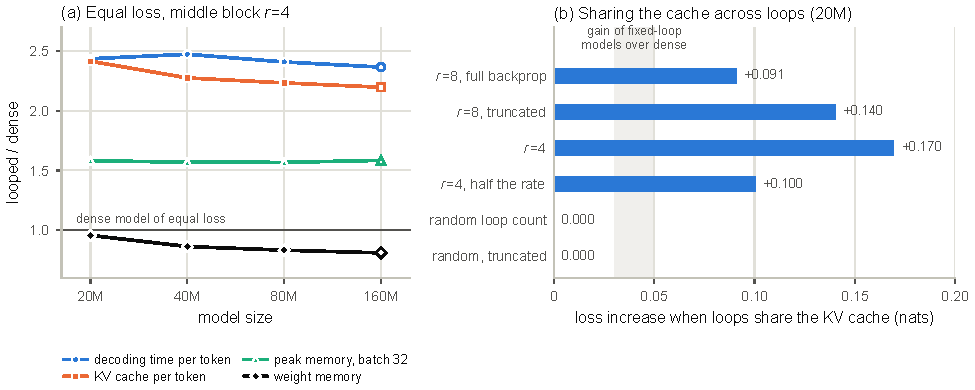
\includegraphics[width=\linewidth]{fig8_deployment}
  \caption{Deployment cost. \textbf{(a)}~A middle block looped 4 times against the dense model of equal loss at $40N$:
  ratios of decoding time per token (batch 1), KV cache per token, peak memory at batch 32 (1k context) and weight
  memory (open markers: 160M lies beyond the largest dense model). \textbf{(b)}~Sharing the KV cache across loops after
  training (20M, one cache slot per unique layer, written at a position's last loop): the loss increase on the main
  set; the shaded band is the fixed-loop models' gain over the dense model of the same size.}
  \label{fig:cost}
\end{figure}

At equal loss, the middle block looped 4 times needs 4\%, 14\%, 17\% and 19\% less weight memory than the dense model
from 20M to 160M (at 160M the dense model of equal loss is extrapolated beyond the largest one trained), but 2.20--2.41 times the KV cache per token and 2.37--2.47 times the decoding time, and its peak
memory at batch 32 is about 1.6 times that of the dense model. At batch 1 the larger KV cache cancels nearly all of the
saving in weights. In this range, loops save parameters, not latency or memory; the saving would grow where weights
dominate memory, for example one sequence with a short context in a much larger model, which we did not test.

Sharing the KV cache across loops would remove most of this cost. We applied terminal sharing, one cache slot per
unique layer written at a position's last loop and read by every later loop, to trained 20M models of one seed
(supplementary experiment S6, \lbl{pre-specified}; Figure~\ref{fig:cost}b). Every model that gains from its loops at this size loses two to four
times that gain: 0.09--0.17 nats against gains of 0.03--0.05 over the dense model, so with a shared cache it would fall
below the dense model of the same size. Truncated backpropagation does not make the cache shareable here, unlike in
\citet{huang2026towards}. The only models that share for free are those trained with a random loop count, whose block
contracts to a fixed point (Section~\ref{sec:mechanism}) and which gain nothing over the dense model. Among the fixed-loop
models, a lower learning rate loses less (0.100 against 0.170 with 4 loops). The likely ways to get sharing are
training towards convergence, or training with the shared cache, which \citet{monea2026shared} find costs no quality;
we tested neither.
